\documentclass[border=4pt]{standalone}
\usepackage{fontspec}
\usepackage{amsmath}
\usepackage{unicode-math}
\setmainfont{Latin Modern Roman}
\setmathfont{Latin Modern Math}
\usepackage{pgfplots}
\usepackage{pgfplotstable}
\pgfplotsset{compat=1.18}
\usepackage{tkz-euclide}
\usetikzlibrary{arrows.meta,calc,angles,quotes,patterns,3d,backgrounds}
\definecolor{ink}{HTML}{123428}
\definecolor{asy}{HTML}{475569}
\definecolor{mint}{HTML}{86e0bd}
\tikzset{asym/.style={asy, line width=0.9pt, dash pattern=on 5pt off 3.5pt},
         guide/.style={gray!70, line width=0.6pt, densely dotted},
         dot/.style={circle, inner sep=0pt, minimum size=5pt, draw=white, line width=0.5pt},
         odot/.style={circle, inner sep=0pt, minimum size=5.5pt, fill=white, line width=1pt},
         lab/.style={font=\footnotesize, inner sep=1.5pt, text=ink}}
\begin{document}
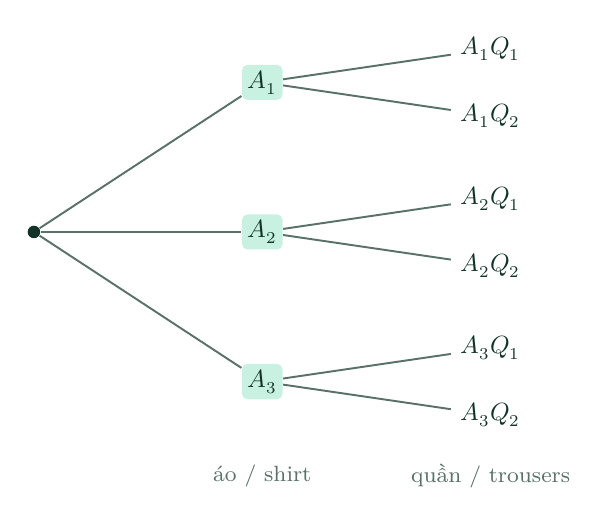
\begin{tikzpicture}[grow=right, level distance=2.9cm, level 1/.style={sibling distance=1.9cm}, level 2/.style={sibling distance=0.85cm},
  every node/.style={font=\small, text=ink}, edge from parent/.style={draw=ink!70, line width=0.7pt}]
\node[circle, fill=ink, inner sep=1.6pt] {}
  child {node[fill=mint!45, rounded corners=2pt, inner sep=2pt] {$A_3$} child {node {$A_3Q_2$}} child {node {$A_3Q_1$}}}
  child {node[fill=mint!45, rounded corners=2pt, inner sep=2pt] {$A_2$} child {node {$A_2Q_2$}} child {node {$A_2Q_1$}}}
  child {node[fill=mint!45, rounded corners=2pt, inner sep=2pt] {$A_1$} child {node {$A_1Q_2$}} child {node {$A_1Q_1$}}};
\node[text=ink!70, font=\footnotesize] at (2.9,-3.1) {áo / shirt};
\node[text=ink!70, font=\footnotesize] at (5.8,-3.1) {quần / trousers};
\end{tikzpicture}
\end{document}
